\section{User Interface}

\subsection{Main Page}

\begin{figure}[H]
    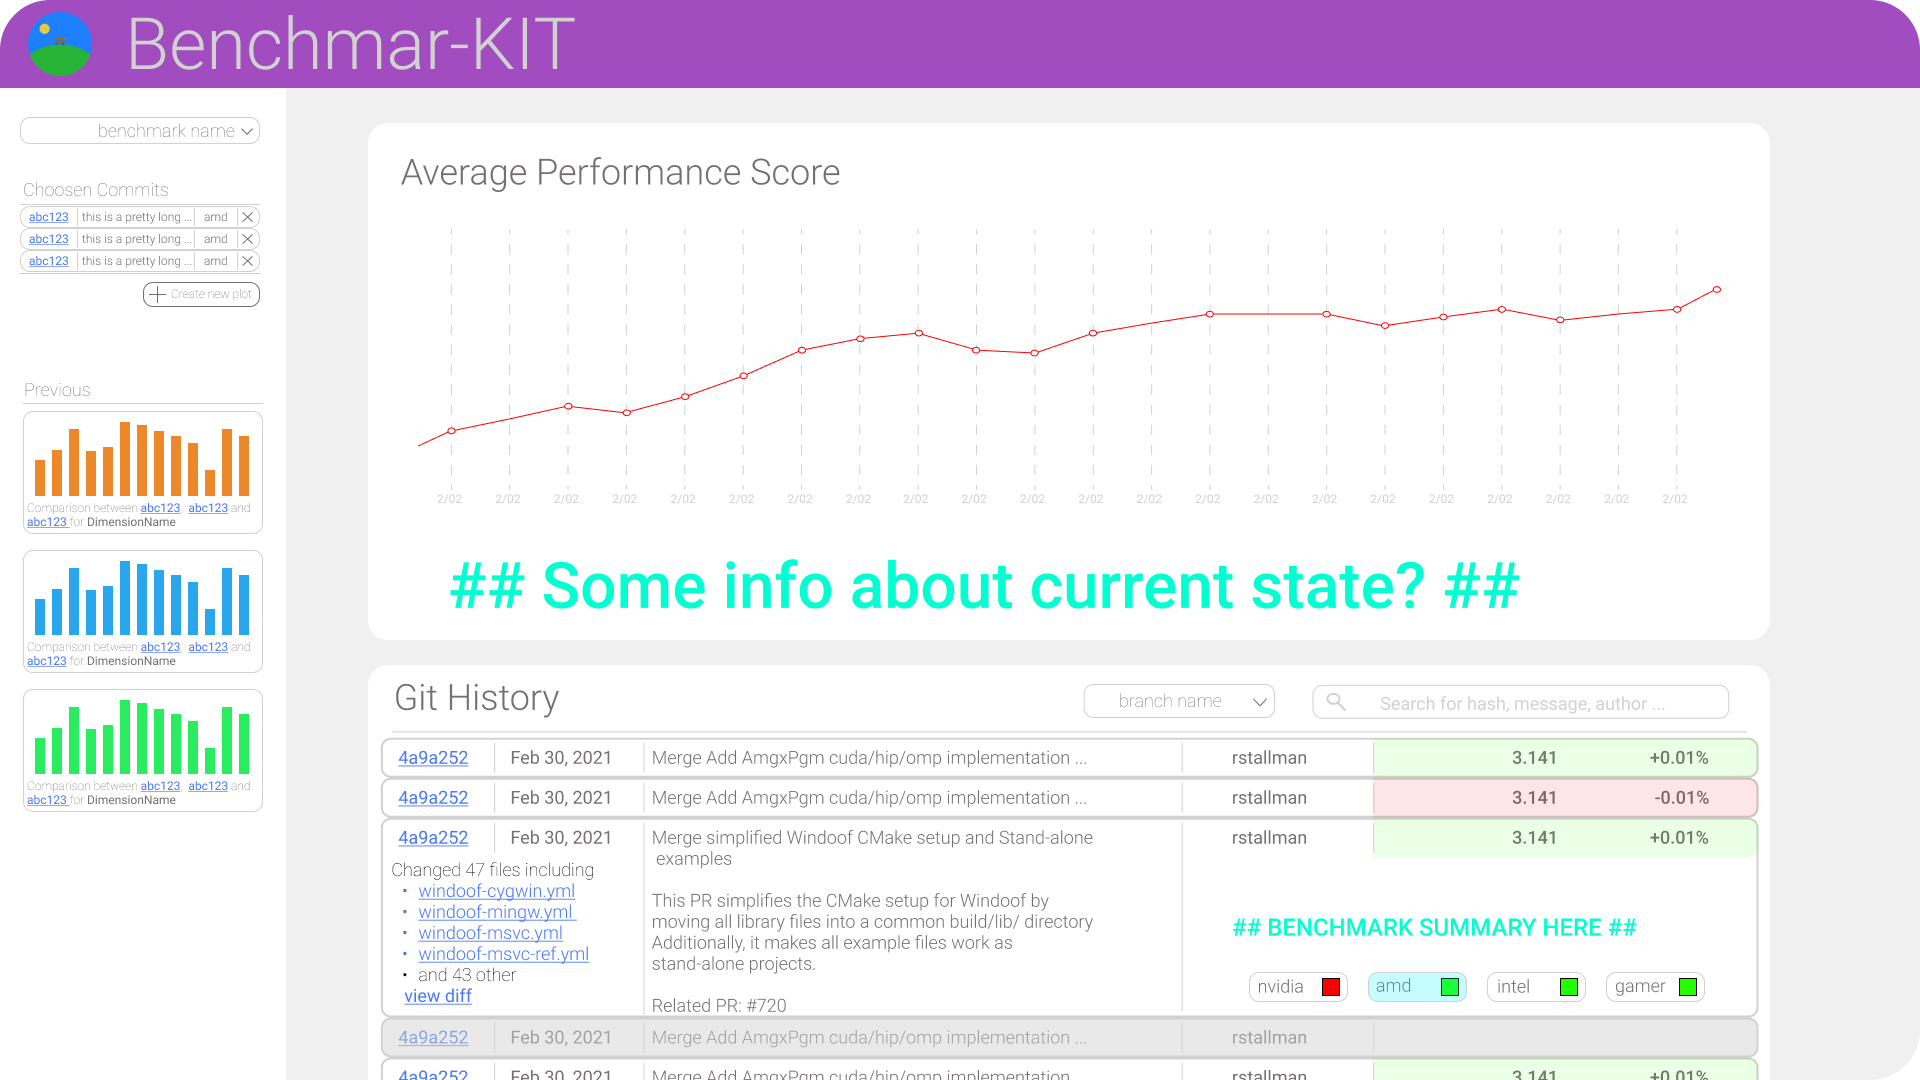
\includegraphics[width=\textwidth]{MainPage.png}
    \caption{Main page}
    \label{ui:main}
\end{figure}

The main page consists of an overview of the commit history, which gets represented by a list of commits. Every entry contains information about the commits such as hash, date and commit message. The user adds commits by selecting a specific commit and then choosing a specific device. Selected commits get added to the list on the left. Benchmark type and branch can be chosen via dropdown menus. The user can open the configuration panel popup by selecting the \enquote{Create New Plot} option.

\subsection{Configuration Panel}

\begin{figure}[H]
    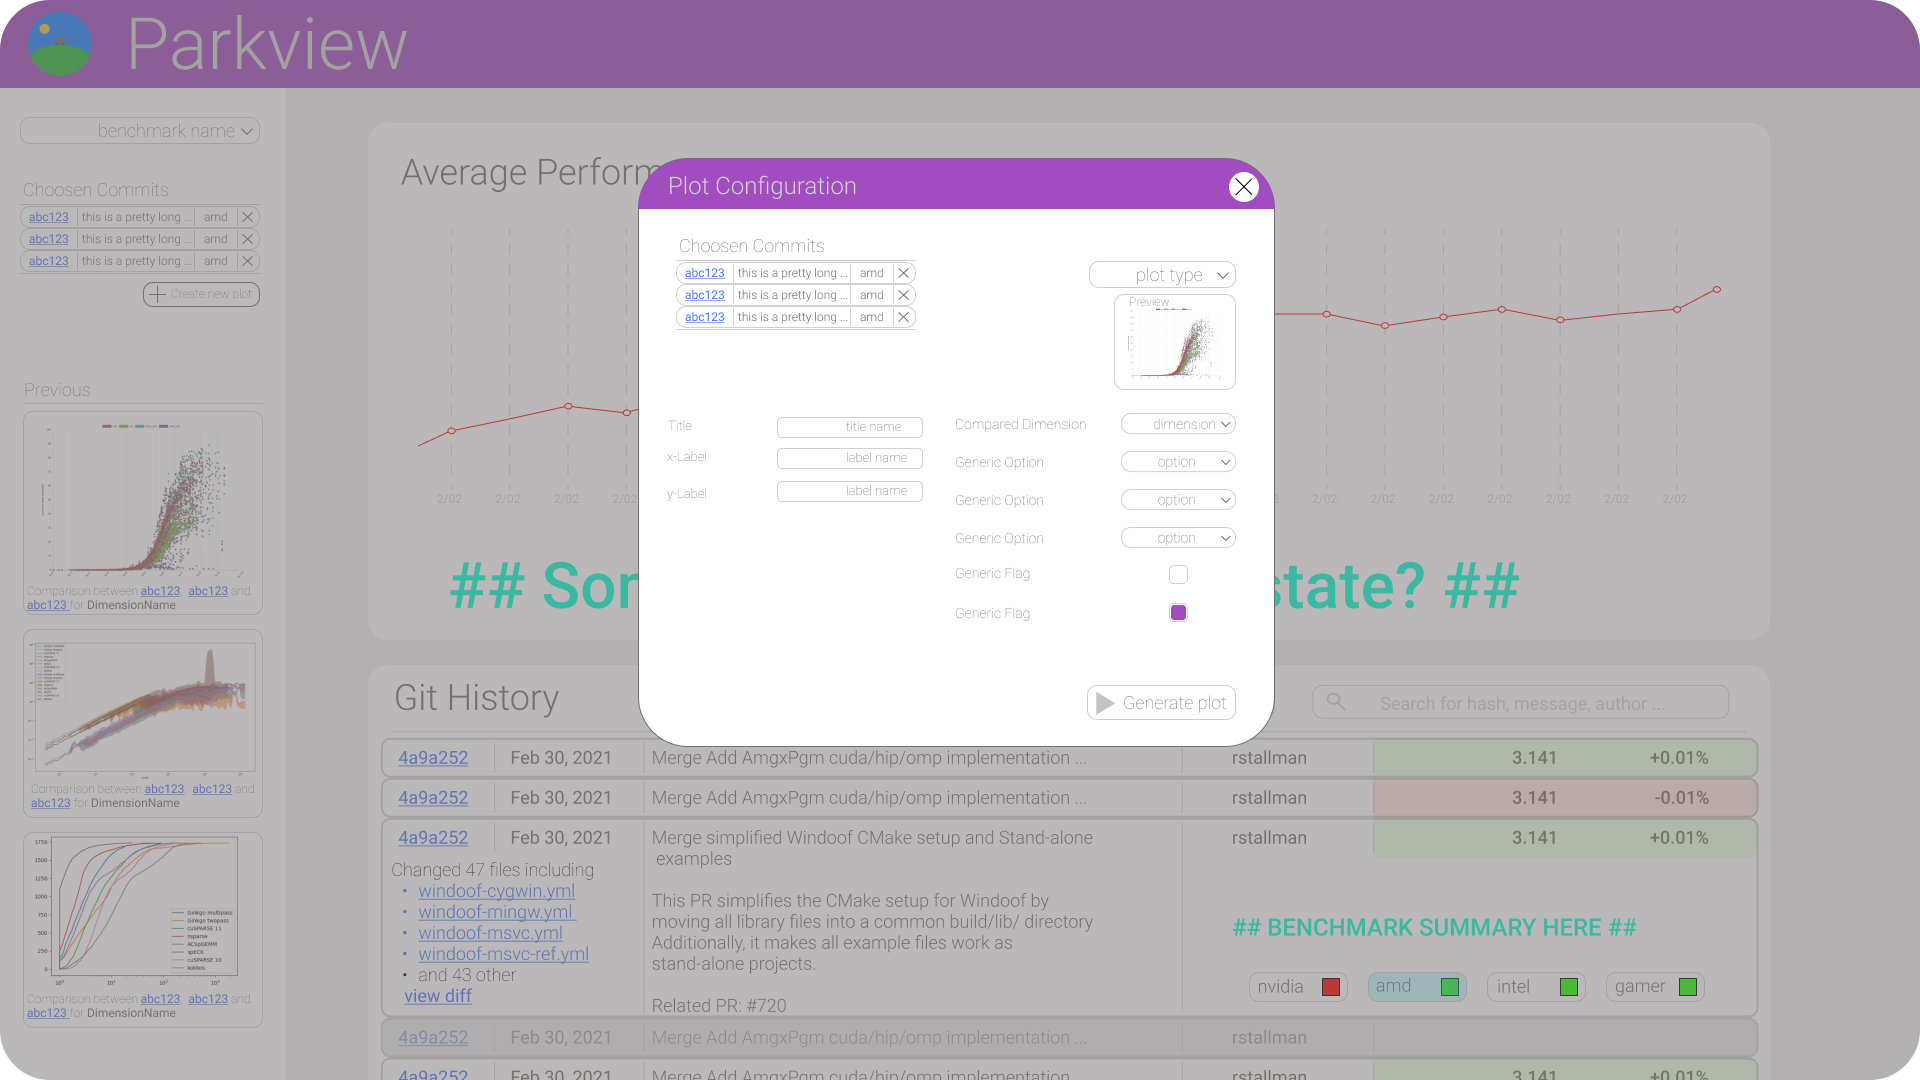
\includegraphics[width=\textwidth]{ConfigurationPopup.png}
    \caption{Configuration Panel}
    \label{ui:config}
\end{figure}

The configuration panel contains all options for configuring the \gls{plot}. Categorical options can be chosen via dropdown menus, flags can be set with checkboxes and any other options can be set using text boxes. The popup can be closed using the cross in the top right. A small preview of the \gls{plot} type gets displayed under the option for \glspl{plot type}. By selecting the \enquote{Generate Plot} option the user starts the generation of the \gls{plot} and the application displays it to the user.

\subsection{Plot View}

\begin{figure}[H]
    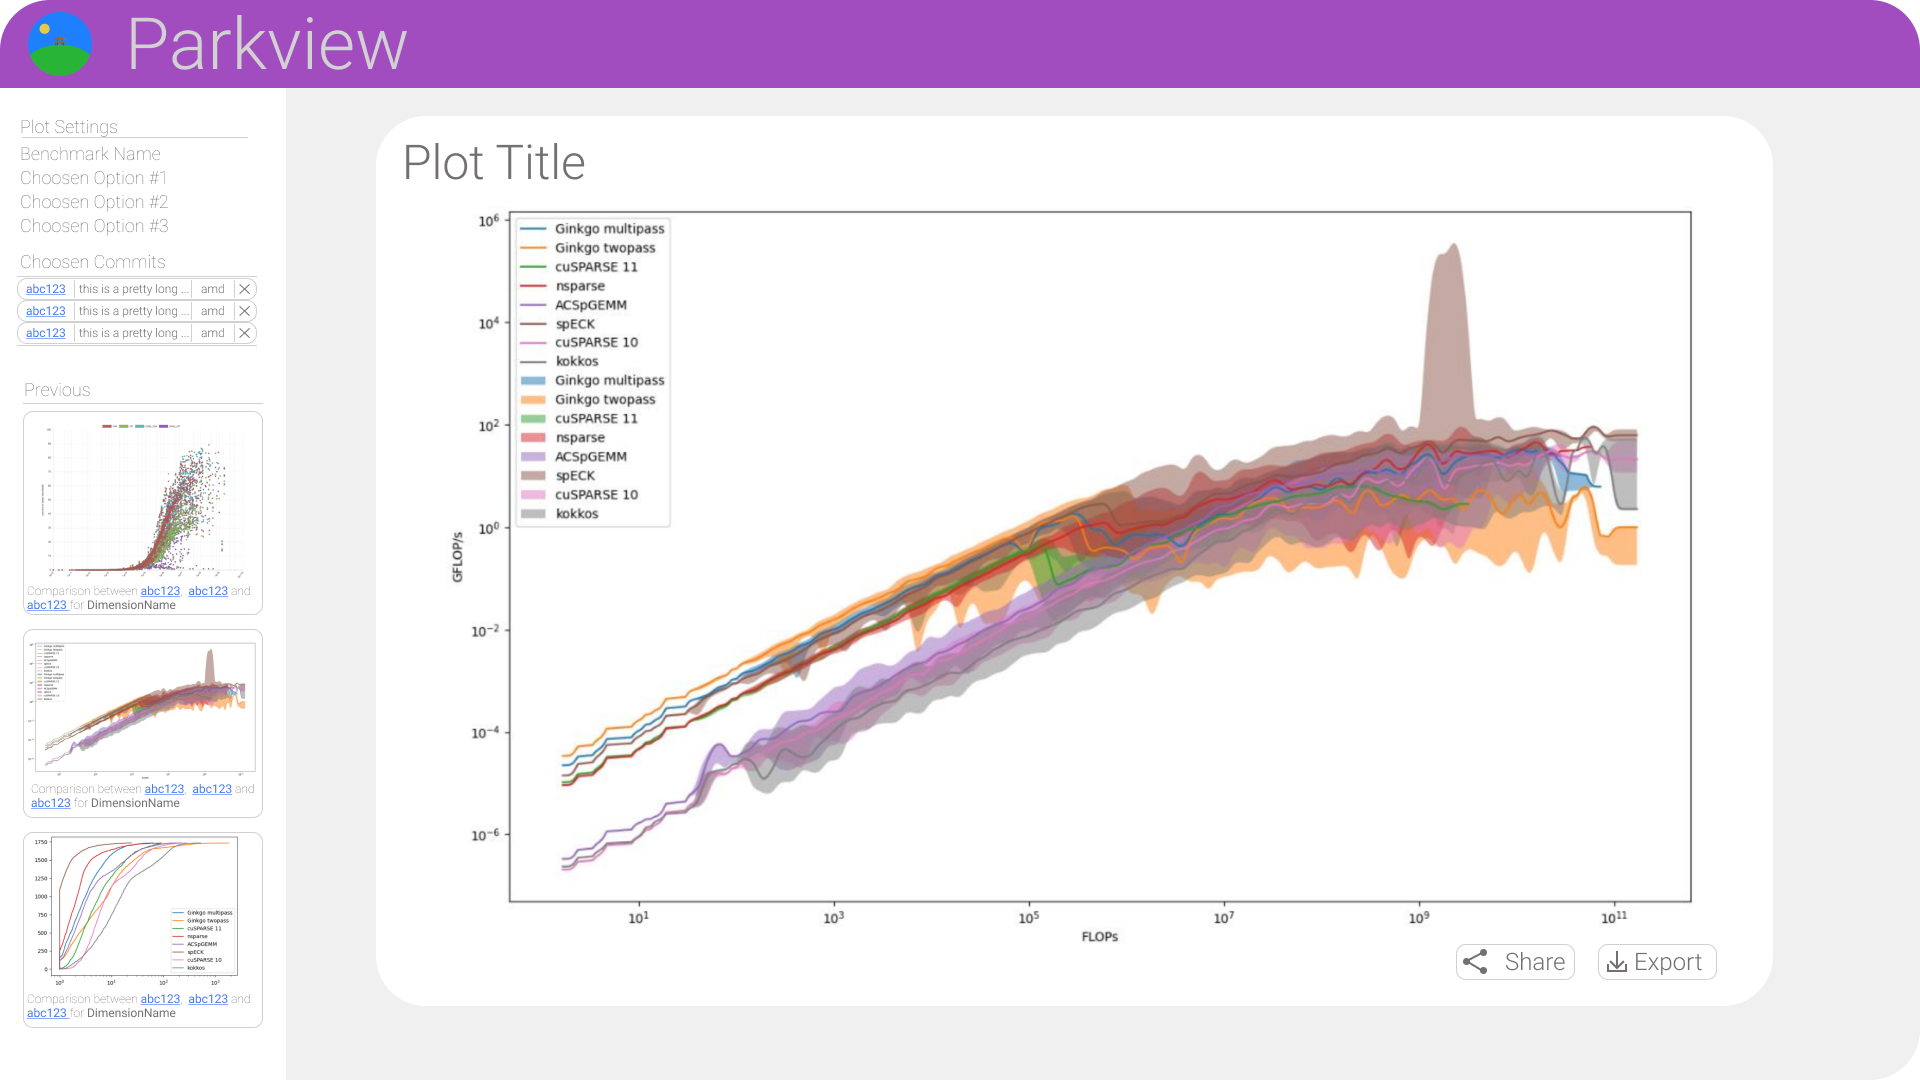
\includegraphics[width=\textwidth]{PlotView.png}
    \caption{View of a \gls{plot}}
    \label{ui:plot}
\end{figure}

The plot view allows the user to inspect the \gls{plot}. The user can share the \gls{plot} by selecting the \enquote{Share} option. He can also download it by selecting the \enquote{Export} option. Selecting the logo on the top left redirects the user to the main page.
